
\chapter{Apéndices}

\section{Apéndice I: Marco referencial}


\subsection{Elaboración de los diferentes apartados del documento}

En la construcción de los marcos referenciales, se consideró iniciar con el marco socio profesional, luego con el marco epistemológico, y, por último, con el marco pedagógico. Sin embargo, tal y como se muestra en el siguiente cuadro, el avance en alguno de los marcos referenciales implicó la revisión continua de los apartados ya trabajados para asegurar, en la medida de lo posible, la coherencia entre cada uno de los aspectos considerados. El apartado histórico del marco socio profesional fue el primero en trabajarse. Durante la redacción del objeto de estudio de la Matemática en el marco epistemológico, surgió la necesidad de reescribir algunos párrafos del marco socio profesional ya construido.  

\begin{table}[H]
\begin{center}
\begin{tabular}{|ll|}
\hline
\multicolumn{1}{|c|}{\cellcolor[HTML]{00C0F3} \textbf{Marco Referencial}} &
\multicolumn{1}{l|}{\cellcolor[HTML]{00C0F3} \textbf{Duración}} \\ \hline
\multicolumn{1}{|l|}{\textbf{Marco socioprofesional}} & \multicolumn{1}{l|}{ \textbf{Enero 2018- Mayo 2020}} \\ \hline
\multicolumn{1}{|l|}{\textbf{Marco epistemológico}} & \multicolumn{1}{l|}{ \textbf{Marzo 2018- Junio 2020}} \\ \hline
\multicolumn{1}{|l|}{\textbf{Marco pedagógico}} & \multicolumn{1}{l|}{ \textbf{Junio 2019-Julio 2020}} \\ \hline
\end{tabular}
\end{center}
\caption{Periodo de trabajo en los marcos referenciales}
\end{table}


En cada uno de los marcos referenciales, cada miembro de la subcomisión fue partícipe en la lectura de la literatura que permitiera comprender el alcance de estos marcos. Luego, a lo interno de la subcomisión, se dedicaron reuniones para analizar los resultados obtenidos y el cómo estos recursos iban a incidir en la construcción del marco que se estaba trabajando. Posteriormente, se estableció cuáles actividades se llevaban a cabo para la obtención de la información, según la realidad de la Escuela de Matemática de la Universidad de Costa Rica. Todo este proceso se acompañó de la constante elaboración de documentos, que requirieron de varios intentos para llegar a su versión. A manera de ejemplo, el análisis estructural de la actividad de álgebra exigió ser trabajado en tres ocasiones, ya que, fue el primero que se diseñó; y, conforme se avanzaba en el proceso de los demás marcos referenciales, se evidenció la necesidad de un ajuste hasta que se logró lo esperado con el aporte de otros miembros de la Escuela, más allá de los miembros de la Comisión. Esta experiencia permitió que la incorporación de otros especialistas fuera considerada desde el principio en los análisis para las demás identidades, lo que permitió agilizar el proceso.

En una etapa avanzada de los marcos referenciales, se extrajo información de los análisis estructurales de la actividad y de los insumos obtenidos a partir de la ejecución de los talleres, con la cual se redactó el perfil de salida y la declaración de los propósitos. Con esta parte concluida, se procede a compartir el documento con la asesora para establecer qué cambios deben trabajarse, con el fin de entregar este documento al Departamento de Matemática, y, posteriormente, a la asamblea de la Escuela de Matemática, con el fin de, en una etapa posterior, llevar a cabo la reestructuración de la carrera en cuestión, objetivo propuesto por esta subcomisión

\section{Marcos referenciales}

En esta sección se fundamenta la propuesta del plan de estudios considerando tres marcos de análisis: el análisis de la profesión, el análisis de la disciplina y el análisis pedagógico. 

\subsection{Análisis de profesión}

En este apartado, se incluyen cuatro componentes que constituyen el marco socio profesional de Matemática: mención de acontecimientos históricos que han permitido el desarrollo de la Matemática en general, cómo ha sido el desarrollo de la Matemática en Costa Rica, qué justifica la oferta académica de esta carrera y la definición profesional de un matemático.  

\subsubsection{Principales hitos de la historia de la Matemática}
 
Este componente histórico pretende situar la forma en la cual esta disciplina ha sido concebida; su revisión aporta elementos de análisis para la posterior elaboración de la malla curricular, así como la identificación de las oportunidades de un matemático en el avance de esta carrera. 

\subsubsection*{El inicio}

Como toda actividad del conocimiento humano, la matemática es fruto de una constante e interesante evolución desde ideas incipientes y desordenadas hasta las sofisticadas estructuras lógicas que la componen en la actualidad. 

Existe evidencia arqueológica, como el Hueso de Ishango y el Hueso de Lebombo, que sugiere que nuestros ancestros han hecho uso de las facultades cognitivas hoy necesarias para la matemática. Sin embargo, no es hasta después de la invención de la escritura, aproximadamente treinta y cinco siglos antes de la era común, que aparece evidencia contundente de un desarrollo de ideas matemáticas sofisticadas.

Durante el milenio siguiente a la invención de la escritura en Sumeria, esta se expande desde el noreste de África hasta la costa este de Asia. Con ella surge el estudio de la matemática en, al menos, cuatro civilizaciones de la era, a las que hoy llamamos Egipto, Babilonia, India y China. La matemática parece alcanzar su apogeo pre-helénico entre los mesopotámicos (babilonios), quienes desarrollan métodos de resolución de ecuaciones lineales y cuadráticas, algoritmos bastante eficientes de aproximación de raíces cuadradas, y, además, encuentran una aproximación de $\pi$ con una precisión equivalente a seis decimales. Cabe destacar que la tableta denominada Plimpton 332, es actualmente la tabla trigonométrica más antigua que se conoce, con casi cuatro milenios de antigüedad.

Una diferencia relevante entre los estudios realizados por estas civilizaciones y aquellos que encontramos por primera vez en el mundo helénico, es la motivación técnica que estos últimos le dieron, estudiándola por sí misma. Los documentos que sobrevi-ven en Mesopotamia (e.g.: Plimpton 332), en Egipto (e.g.: el Papiro de Ahmes) y China (e.g.: el Zoubi) son esencialmente libros de texto, donde se expresa el uso de la mate-mática como una herramienta, y no como un campo de estudio por su propio mérito. En India, los textos en los que encontramos relaciones con matemática (sulbasutras), como muchos otros textos de la época en esta región, se escriben en verso, para ser declamados o cantados. Este estilo de escritura dificulta la inclusión del desarrollo técnico del área de estudio

\subsubsection*{El mundo helénico}

Para el inicio del primer milenio (a. e. c.), existía un número importante de ciudades a lo largo de todo el Mediterráneo, que alberga la diáspora helénica (poblaciones étnica y culturalmente griegas, pero sin nexo político con las ciudades en lo que llamamos actualmente Grecia). Es en una de estas ciudades, en Mileto, donde en el siglo VII AEC nace Thales, quien además de ser quizá el primer gran filósofo occidental, entre otros logros loables, es también la primera persona que, mediante el uso de un sistema axiomático deductivo, realiza demostraciones en geometría. 
Es uno de los discípulos de Thales quien décadas después iniciaría una academia a la que se le atribuyen un número importante de resultados en geometría, estereometría y teoría de números. Tanto es así, que el teorema más famoso en matemática, es conocido con el nombre de este sabio: Pitágoras.

Posteriormente, tanto los descendientes intelectuales de Pitágoras, como los matemáticos alejandrinos, producen una serie de descubrimientos teóricos muy relevantes: la inconmensurabilidad de la diagonal del cuadrado, los problemas clásicos de la duplicación del cubo, la trisección del ángulo y la cuadratura del círculo.

Durante el siglo IV a.e.c, en Alejandría, aparecen los trece libros de los Elementos de Euclides, que reinaría supremo como texto matemático por casi dos milenios. En el siglo siguiente, un número importante de matemáticos trabaja en Alejandría, con la excepción importante de Arquímedes, quien lo hace desde su natal Siracusa. Este último desarrolla, por primera vez, técnicas de cálculo de tangentes para curvas no circulares, que son reconocibles como precursores del cálculo diferencial. También desarrolla el método de exhaución, ancestro intelectual directo del cálculo integral.

Son innumerables los otros avances que encontramos emanando de Alejandría hasta principios del siglo V de la era común, incluyendo los estudios de cónicas de Apolonio, que inspiraron a Descartes milenio y medio después a desarrollar su geometría analítica, o el universo de Tolomeo, modelo astronómico dominante hasta el siglo XVII, destronado por los trabajos de Copérnico, Bruno, Galileo, Brahe y Kepler. 

\subsubsection*{La edad media}

Tras la caída del Imperio Romano de Occidente, en el 476 de la e.c., el epicentro del avance académico pasa del mundo helénico, a India y al Islam. En India se perfecciona el sistema de notación posicional babilónico, se introduce el concepto del cero, se perfecciona el cálculo de lo que hoy denominamos funciones trigonométricas, entre otros logros.

Mientras tanto, los califas del mundo islámico reconocen la constante pérdida de conocimiento en occidente, e inician hacia el siglo VIII la preservación y traducción al árabe de las obras clásicas.

Durante el siglo IX, al-Khwarizmi desarrolla un sistema de notación, el cual publica alrededor del año 833 de la e.c., en su libro Compendio de cálculo por reintegración y comparación, usualmente referido por su abreviación en árabe, al-gebr. Del nombre del autor tenemos la palabra algoritmo, y de su obra, la palabra álgebra.

Durante el siglo XI, Omar Kayyam encuentra y generaliza el método de cálculo de raíces de ecuaciones cúbicas mediante la reducción del problema a la intersección entre dos secciones cónicas. Esta técnica puede ser aplicada en algunos pocos casos en ecuaciones de grado mayor a tres. 

Los avances en teorías matemáticas fueron pocos y esporádicos durante el milenio al que denominamos la edad media. Esto es particularmente evidente en Europa. Sin embargo, la matemática, en el viejo continente, no fue completamente estéril durante este periodo. Leonardo de Pisa, conocido como Fibonacci, es quizá la figura más conocida del periodo. A lo largo de su vida, durante el final del siglo XII y el inicio del XIII, su obra se encargó de popularizar el sistema de numeración indo-arábico en occidente. Además, a pesar que la mayor parte de los resultados en sus obras parecen ser obtenidos directamente de los clásicos, o de obras del mundo árabe, la mayor parte de sus demostraciones son originales.

Otras figuras relevantes en la matemática de la Europa medieval son Nicole Oresme, en el siglo XIV, y Luca Pacioli, en el XV. Oresme explora técnicas de resolución de sistemas de ecuaciones lineales y cuadráticas en dos o tres variables, además de explorar —dicho sea de paso, con una matemática profundamente insuficiente— la dispersión del calor en varillas y platos metálicos. Por otro lado, Pacioli, a quien se le conoce como el padre de la contabilidad, publica obras en las cuales detalla métodos contables, interés y otras habilidades matemáticas útiles al mercader.

También, durante el siglo XV, el arquitecto florentino, Filippo Brunelleschi, desde la perspectiva del diseñador y el artista, desarrolla algunas de las ideas básicas de la geometría perspectiva, que serían formalizadas siglos después. 

\subsubsection*{El Renacimiento}

En 1545, Gerolamo Cardano publica su libro Ars Magna, el cual contiene la primera fórmula general para la resolución de la ecuación cúbica. Este es, quizá, el primer descubrimiento matemático trascendental en Europa en un milenio, e incentivó el interés por los números complejos y estimuló la búsqueda de soluciones para ecuaciones de quinto grado y superior.

Durante este siglo se populariza el uso de notación algebraica precursora de la moderna. El matemático francés François Viète llevó a cabo estudios importantes sobre la resolución de 
ecuaciones.

\subsubsection*{El siglo XVII}
 
A inicios del siglo XVII, el matemático escocés John Napier introduce el concepto de logaritmo. Unas décadas después, Pierre de Fermat realizó importantes descubrimientos en la teoría de números, incluyendo su famosa conjetura conocida como último teorema de Fermat, que serviría de inspiración para una gran cantidad de trabajos en álgebra y teoría de números. Esta conjetura fue demostrada por Andrew Willes a finales del siglo XX.

En 1637, René Descartes publica su ensayo el Discurso del método, el cual, además de ser la base filosófica para el desarrollo del método científico, también contiene tres apéndices: Dióptica, Meteórica y Geometría. El último mencionado se considera el trabajo inaugural en geometría analítica, que serviría, como base para el desarrollo del cálculo medio siglo después.

También en el área de geometría, el ingeniero francés, Gérard Desargues, posiblemente inspirado en la obra de Brunelleschi de dos siglos atrás, formaliza los conceptos básicos de la geometría proyectiva.

Durante la Gran Plaga de Londres, de 1665 a 1666, Isaac Newton, con tan sólo 22 años de edad, desarrolla los conceptos básicos del cálculo integral y diferencial. Sin embargo, no sería hasta 1684, que, inspirado por una conversación con Edmond Halley, reconstruye sus ideas de dos décadas atrás y se las envía. Halley describe esta carta como las primeras páginas de la ciencia moderna. 

Sin embargo, al otro lado del canal, el filósofo y matemático autodidacta Gottfried Leibniz desarrolla, de manera independiente, entre 1675 y 1684, una teoría análoga a la de Newton, la cual publica antes que el inglés. Esto iniciaría una de las disputas científicas más infames en la historia de las ciencias. 

\subsubsection*{El siglo XVIII}

Durante el siglo XVIII, se desarrollaron nuevos campos dentro de la matemática, en gran parte como respuesta a la teoría del cálculo diferencial e integral y sus aplicaciones.

Los hermanos Bernoulli desarrollaron el cálculo de variaciones y el matemático francés Gaspard Monge la geometría descriptiva. Joseph-Louis Lagrange dio un tratamiento analítico de la mecánica en su gran obra Mecánica analítica (1788), en donde se pueden encontrar las famosas ecuaciones de Lagrange para sistemas dinámicos. Además, Lagrange hizo contribuciones al estudio de las ecuaciones diferenciales y la teoría de números, y desarrolló la teoría de grupos. 

El gran matemático del siglo XVIII fue el suizo Leonhard Euler, quien aportó ideas fundamentales sobre el cálculo y otras ramas de las matemáticas y sus aplicaciones. Euler escribió textos
sobre cálculo, mecánica y álgebra que se convirtieron en modelos a seguir para otros autores interesados en estas disciplinas. Todos estos avances acentuaron la necesidad de un estudio más formal
del cálculo, necesidad que sería respondida hasta el siglo posterior. 

\subsubsection*{El siglo XIX}

En 1812, Pierre Laplace publica el libro Teoría analítica de las probabilidades, donde formaliza muchos de los conceptos que fueron utilizados empíricamente por figuras como Fibonacci o Cardano. Además, durante el primer cuarto de este siglo escribe los cinco volúmenes de su Tratado de la mecánica celeste.

A Augustin-Luis Cauchy se le atribuye la incorporación de un enfoque lógico y apropiado del cálculo. Su visión del cálculo se basaba solamente en cantidades finitas y el concepto de límite.
Nace con esto la necesidad de una definición lógica de número real.

Fue el matemático alemán Julius W. R. Dedekind quien encontró una definición adecuada para los números reales, a partir de los números racionales, que todavía se enseña en la actualidad.
Los matemáticos alemanes Georg Cantor y Karl T. W. Weierstrass también dieron otras definiciones casi simultáneas. 

En esta época surge también el problema de definir el significado de la palabra función. Joseph-Louis Lagrange y Joseph Fourier aportaron soluciones, pero fue el alemán Peter  G. L. Dirichlet quien propuso su definición en los términos actuales. 

Además de fortalecer los fundamentos del análisis, los matemáticos del siglo XIX llevaron a cabo importantes avances en esta materia. A principios del siglo, Carl Friedrich Gauss dio una explicación adecuada del concepto de número complejo, con lo cual se forma un nuevo campo del análisis matemático (y del álgebra), desarrollado en los trabajos de Cauchy, Karl Weierstrass y su propio discípulo, el matemático alemán Bernhard Riemann. 

Otro importante avance del análisis fue el estudio, por parte de Fourier, de las sumas infinitas de expresiones con funciones trigonométricas, conocidas actualmente como series de Fourier.  El análisis de Fourier llevó también a Cantor al estudio de los conjuntos infinitos y a una aritmética de números infinitos. La teoría de Cantor, que fue muy criticada en la época, forma hoy parte de los fundamentos de las matemáticas. 

Otro descubrimiento controversial y ampliamente criticado del siglo XIX fue la geometría no euclídea. Aunque descubierta primero por Gauss, este tuvo miedo a la controversia. Los mismos resultados fueron descubiertos y publicados por el matemático ruso Nikolái Ivánovich Lobachevski y por el húngaro János Bolyai. Las geometrías no euclídeas fueron estudiadas en su forma más general por Riemann, con su descubrimiento de las múltiples paralelas. En el siglo XX, a partir de los trabajos de Einstein, se le han encontrado también aplicaciones en Física. 

Gauss es considerado uno de los más importantes matemáticos de la historia. Su libro Disquisitiones arithmeticae (1801) marcó el comienzo de la era moderna. En su tesis doctoral presentó la primera demostración apropiada del teorema fundamental del álgebra. Pero más importante aún fue la transformación que sufrió el álgebra durante el siglo XIX, debido a que pasó del simple
estudio de los polinomios al estudio de la estructura de sistemas algebraicos. Otro paso importante fue el desarrollo de la teoría de grupos, a partir de los trabajos de Lagrange. Evariste Galois utilizó estos trabajos para desarrollar su teoría de polinomios resolubles.

Los fundamentos de las matemáticas se vieron también transformados durante el siglo XIX, sobre todo por el matemático inglés George Boole que algebrizó la lógica clásica mediante las álgebras de Boole. También la teoría de Cantor de cardinales, impulsó la teoría de conjuntos moderna. 

Hacia finales del siglo, se descubrieron una serie de paradojas en la teoría de conjuntos cantoriana dada por la axiomática de Gottlob Frege. El matemático inglés Bertrand Russell encontró una de estas paradojas, que afectaba al propio concepto de conjunto. Los matemáticos resolvieron este problema por medio nuevas axiomatizaciones de la teoría de conjuntos que eliminan las paradojas conocidas. Sin embargo, no se ha podido comprobar la consistencia de estas nuevas axiomatizacines. Hasta nuestros días, solo se han encontrado demostraciones relativas de consistencia (si la teoría B es consistente entonces la teoría A también lo es). Este sistema axiomático, comúnmente aceptado, es el de Zermelo-Fraenkel. También existen otras axiomáticas de la teoría de conjuntos dadas por Neumann-Bernays-Gödel. 


\subsubsection*{La matemática moderna (inicios del siglo XX y la aparición de computadoras)}

David Hilbert fue uno de los matemáticos más sobresalientes de finales del siglo XIX y la primera mitad del siglo XX, ya que había contribuido de forma sustancial en casi todas las ramas
de las matemáticas, desde su clásico Fundamentos de la geometría (1899) a su Fundamentos de la Matemática en colaboración con otros autores. 

En la Conferencia Internacional de Matemáticos de París en el año 1900, Hilbert dio una lista de veintitrés problemas que a su juicio ocuparían la mente de los matemáticos durante el siglo XX. Y en efecto, así fue; estos problemas estimularon gran parte de los trabajos matemáticos del siglo XX, y cada vez que aparecen noticias de que otro de los “problemas de Hilbert” ha sido resuelto, la comunidad matemática internacional espera los detalles con inquietud. 

Los teoremas de completitud e incompletitud de Kurt Gödel (alrededor del año 1930) resuelven un problema de Hilbert, al desarrollar, de manera moderna, la lógica matemática con la noción de verdad de Alfred Tarski y la reformulación del teorema de completitud. Esto constituye el nacimiento de la teoría de modelos. El teorema de incompletitud de Gödel demostró que, cualquier sistema de axiomas que extiende (de manera consistente) la aritmética, es indecidible; es decir, que es posible encontrar proposiciones cuya certeza no se puede demostrar ni refutar dentro
del sistema.

Alrededor de 1920, Emmy Noether brindó los fundamentos modernos del álgebra mediante sus teoremas de isomorfismo y la teoría de ideales en anillos (iniciada por Ernst Kummer). En la siguiente década, Emil Artin y Otto Schreier dieron solución al problema 17 de Hilbert. Esto llevó al surgimiento de la teoría de primer orden de los números reales y constituyó el fundamento de la
geometría algebraica real.

Posteriormente, David Hilbert da los primeros pasos en la algebrización de la geometría con sus teoremas de la base y teorema de ceros. Esto permitió el inicio del estudio de la geometría a través del álgebra conmutativa (Oscar Zariski, Pierre Samuel, entre otros). Alexander Grothendieck da los fundamentos modernos de la geometría algebraica (clásica) por medio del uso de la teoría de haces (Jean-Louis Loday) y al introducir los esquemas, en la década de los 60 en el IHES. 

Aunque los orígenes de las computadoras fueron las calculadoras de relojería de Pascal y Leibniz en el siglo XVII, fue el inglés Charles Babbage quien, en el siglo XIX, diseñó una máquina capaz de realizar operaciones matemáticas automáticamente. La imaginación de Babbage sobrepasó la tecnología de su tiempo, y no fue hasta la invención del relay, la válvula de vacío y después la del transistor cuando la computación programable a gran escala se hizo realidad. 

Este avance ha impulsado ramas de las matemáticas, como el análisis numérico y las matemáticas finitas, y ha generado nuevas áreas de investigación como el estudio de los algoritmos. Se ha convertido en una herramienta poderosa en campos tan diversos como la teoría de números, las ecuaciones diferenciales y el álgebra abstracta. Además, la computadora ha permitido encontrar la solución a varios problemas matemáticos que no se habían podido resolver anteriormente, como el problema topológico de los cuatro colores, propuesto a mediados del siglo XIX. Este teorema fue demostrado en 1976, al utilizar una computadora de gran capacidad de cálculo en la Universidad de Illinois. 

Así como la computación ha ayudado a encontrar soluciones de problemas irresolutos en la matemática, también la computación ha reforzado las matemáticas a apegarse al constructivismo promulgado por Brower; esto por cuanto la existencia de ciertos objetos matemático-computacionales necesita ser explícita mediante procesos que los construyan (algoritmos) y no mediante su mera existencia. Un ejemplo en este sentido está constituido por el teorema de ceros de Hilbert. Este lo demostró de manera no constructiva, y actualmente existen centenas de artículos sobre la
efectividad de este resultado. Lo anterior está íntimamente ligado a la lógica intuicionista (Heyting, Troelstra, etc.), por lo cual, la demostración de un enunciado existencial en esta lógica da forzosamente la construcción del objeto. 

Hoy el conocimiento matemático avanza más rápido que nunca. Teorías que tenían muy poca relación entre sí se han unido para formar otras más completas y abstractas. Muchos problemas importantes han sido resueltos, pero otros siguen sin solución. Al mismo tiempo siguen apareciendo problemas nuevos e interesantes. Incluso las matemáticas más abstractas están encontrando aplicaciones. La teoría de números y teoría de curvas elípticas (geometría algebraica) que son sumamente abstractas son fundamentales para la encriptación. El álgebra se ha venido estudiando desde el punto de vista de la constructibilidad para dar nacimiento a un álgebra computacional fundada principalmente en las bases de Groebner. También han surgido métodos computacionales en la geometría algebraica real dada por la descomposición cilíndrica de Collins desarrollada en los años 70 (mejor algoritmo para la decidibilidad de la teoría de los números reales) y sus subsiguientes algoritmos.

\subsubsection{Historia del desarrollo de las matemáticas en Costa Rica}

Desde sus inicios en el país, cuando se han realizado transformaciones en la forma de transmitir la matemática a otros, ha prevalecido una intención. En el contexto de la reestructuración de la carrera, se observa lo sucedido en años anteriores y se concuerda que el contexto y las oportunidades disponibles son esenciales para la toma de decisiones correspondiente

\subsubsection*{Inicios de la educación universitaria en Costa Rica. La Universidad de Santo Tomás}

En la Costa Rica colonial, la educación no era prioridad alguna. El primer indicio de enseñanza data del año 1594, con la existencia de una escuela elemental en Cartago, donde la instrucción se fundamentaba en la escritura, lectura, conteo y doctrina cristiana. A nivel de educación primaria y secundaria, los gobernantes costarricenses dieron prioridad especial al desarrollo educativo, paulatinamente, con lo cual destaca, por ejemplo, una reforma en 1849 del gobierno del Dr. José María Castro Madriz que conlleva la creación de una escuela normal, un liceo para niñas y una reestructuración de la educación primaria. Posteriormente, un hito histórico relevante es la incorporación de la enseñanza primaria gratuita, obligatoria y costeada por el Estado en la Constitución en 1869. 

El primer antecedente de educación universitaria corresponde a la Casa de Enseñanza de Santo Tomás, creada en 1814 bajo la rectoría del Bachiller Rafael Francisco Osejo. Contaba con clases de primeras letras donde se aprendía a leer y escribir, a contar, junto con clases de Filosofía, de Gramática Castellana y Latina. En 1830, el Bachiller Osejo terminó de redactar su libro, Breves lecciones de aritmética, utilizado para enseñar matemática, el cual incluía también geometría. Tenía un nivel elemental, con claridad y orden, y era utilizada en primaria y primeros años de secundaria.

Luego de distintas reformas y reorganizaciones, en el año 1824 la institución adquirió un verdadero carácter preuniversitario donde se establece el grado de Bachiller, pero hasta 1838 se presentaron las primeras solicitudes de graduación de Bachiller en Filosofía. Según Paulino González, en su libro La Universidad de Santo Tomás, la enseñanza de la matemática en la Universidad  de Santo Tomás aparece hasta 1846. Ya en 1848, la Cátedra de Matemáticas existía y contaba en ese año con dieciséis alumnos. En 1849, aritmética, álgebra y geometría eran parte de las materias en las que los aspirantes al grado de Bachiller en Filosofía y Humanidades debían rendir examen. 

Desde los primeros años, había dentro de la Universidad de Santo Tomás una escuela primaria y era usual pasar de la escuela primaria a clases universitarias de manera directa. 

En 1861, se declararon como universitarias las Cátedras de Filosofía y Matemáticas, con una tendencia clara por establecer carreras técnicas aplicadas a la agrimensura y artesanía nacional, en las cuales se impartía un curso de dibujo (artístico y técnico). Además, el país necesitaba personal capacitado en estudios específicos en ingeniería para la construcción de puentes y caminos. Así, en 1869 se incluyen estudios de ingeniería civil, arquitectura y la agrimensura. Este programa incluyó la primera referencia a la enseñanza del cálculo en nuestro país. Sin embargo, la Cátedra de Matemáticas cerró debido a la apertura de estas carreras. Finalmente, en 1888 se aprobó la clausura de la Universidad de Santo Tomás, al aducir que no respondía a las necesidades de la sociedad costarricense en ese momento. 

\subsubsection{La reforma de Mauro Fernández y las matemáticas}

Mauro Fernández fue nombrado como máxima autoridad de la Secretaría de Instrucción Pública en 1885 por el entonces presidente Bernardo Soto. Fernández propició una reforma a la
educación del país, cuyo objetivo primordial era reorganizar la enseñanza primaria, organizar una buena segunda enseñanza y reorganizar la Universidad, acorde con las necesidades de la sociedad costarricense. La educación en Costa Rica fue el principal instrumento social con el que se buscaba solidificar la identidad nacional y afianzar las relaciones entre las clases sociales. Esta fue una de las banderas de lucha y un instrumento político de los grupos sociales y políticos liberales.

Dicha reforma culmina con la Ley General de Educación Común en 1886. Parte de la reforma incluía además la formación y capacitación de los docentes, así como su mejor remuneración. Tenía el pensamiento que “el gobierno debía reformar la Universidad de una manera significativamente diferente; de hecho, pensaba en términos de un politécnico al estilo francés, donde las ciencias y las técnicas ocuparían el lugar fundamental, pero primero debía darse la completa reorganización de la primaria y de la segunda enseñanza, base de la educación superior”, (cf. [17]).

\subsubsection{Los programas de Matemáticas en la enseñanza primaria y secundaria entre 1886 y 1940}

Las crecientes exportaciones y las consecuentes mejoras en la economía permitieron invertir en educación, generando un incremento en el número de escuelas y docentes. No obstante, la calidad de la educación no era la mejor, lo cual se reflejaba en una alta deserción escolar. En 1908, se definieron nuevos programas de estudio, los cuales fueron realizados por Roberto Brenes Mesén y Joaquín García Monge, pero, debido a la oposición de grupos conservadores, solo duraron un año. 

No obstante, se inició a:

        “dar prioridad a la participación efectiva de la escuela, no solo como institución de desarrollo del niño, sino también como pivote de la economía; promoviendo la educación como medio de participación en el desarrollo nacional. De ahí la importancia que se le dio al desarrollo de la escuela rural, que fue concebida como centro de creación de riqueza agrícola e industrial.”

Así, se hizo una diferenciación en la metodología al enseñar Aritmética y Geometría en zonas rurales, en la cual se hace hincapié en que los ejercicios y problemas debían estar orientados a las necesidades de las comunidades rurales. 

También, producto de la rebelión contra la dictadura de los Tinoco, se aumentó el presupuesto para la educación, al eliminar gastos militares. Algo similar ocurrió posteriormente con la abolición del ejército, lo cual da una visión país donde la educación se convierte en un elemento de vital importancia para el desarrollo económico e integral de los ciudadanos, donde se proporciona un mínimo de conocimientos a la población (leer, escribir y contar).

\subsubsection*{La Escuela Normal y las matemáticas hasta la creación de la Universidad de Costa Rica}

La formación de maestros en nuestro país se puede dividir en seis etapas diferentes:

\begin{itemize}

  \color{blue}  \item \color{black} A partir del Reglamento Orgánico de Instrucción Pública de 1849, artículo 254, se plantea la idea de una Escuela Normal en San José para la formación de maestros (escuela primaria superior).
    
   \color{blue} \item \color{black} La Reforma de Mauro Fernández, con la creación de las Secciones Normales del Liceo de Costa Rica y el Colegio Superior de Señoritas (nivel de secundaria).
    
    \color{blue} \item \color{black} En 1914 se crea la Escuela Normal en Heredia (preparación postsecundaria, y dos años para la especialidad en enseñanza primaria), con el objetivo de mejorar la formación de maestros
    
    \color{blue} \item \color{black} En 1936 se hace una reforma de la Sección de Humanidades en la Escuela Normal.
    
    \color{blue} \item \color{black} La creación de la Universidad de Costa Rica, en donde se organiza la Escuela de Pedagogía y se elevó la formación de maestros a nivel universitario. 
    
    \color{blue} \item \color{black} La Reforma Universitaria de 1957 convierte a la Escuela de Pedagogía en la nueva Facultad de Educación. 
\end{itemize}


De esta manera, todas las reformas atendían a las necesidades de la época, donde el fin era mejorar la formación de maestros, tanto para educación primaria y secundaria. Las escuelas anexas del Liceo de Costa Rica y del Colegio Superior de Señoritas desaparecen con la creación de la Escuela Normal, lo cual la lleva a convertirse en la única responsable en la preparación de los
educadores costarricenses. La Sección Pedagógica se conformó como una escuela profesional dedicada a formar maestros y profesores. Con la creación de la Universidad de Costa Rica, la Sección de Pedagogía pasó a ser la Escuela de Pedagogía de la Universidad, sin mayores cambios en su vida institucional. 

 \subsubsection*{ Las matemáticas en la Escuela de Ciencias de la Universidad de Costa Rica }
 
Cuatro circunstancias definieron el marco institucional y el espacio académico nacionales donde se desarrollarían las matemáticas universitarias en la segunda mitad del siglo XX: la creación de la Universidad de Costa Rica, en 1940; la Reforma Universitaria de Rodrigo Facio, en 1957; el Tercer Congreso Universitario de la UCR, en 1972-1973; y, la creación de tres nuevas universidades estatales en la década de los setenta: la Universidad Nacional, el Instituto Tecnológico de Costa Rica
y la Universidad Estatal a Distancia.

Con la creación de la Universidad de Costa Rica en 1940, se estableció la Escuela de Ciencias, donde las matemáticas no eran una disciplina independiente, sino más bien satisfacía las necesidades de otras carreras. En particular, uno de sus mayores objetivos era la formación de profesores para enseñanza media. A finales de la década de los 40, el número de estudiantes era bajo, y para la década siguiente se ofreció un plan de estudios con énfasis en Física y Matemática, cuyo título correspondía al de Profesor de Enseñanza Media. 

 \subsubsection*{El Departamento de Física y Matemáticas }

En 1957, inició el funcionamiento del Departamento de Física y Matemáticas, momento en el cual se integran al departamento casi todos los cursos de matemáticas que se impartían en diferentes unidades académicas, siendo el principal antecedente de la creación posterior de la carrera de matemáticas. 

Durante los años 1961-1962, los planes de estudios del Departamento estaban plenamente adaptados a la Reforma y entrelazan Física y Matemáticas. Muchos estudiantes buscaban obtener el título de Profesor de Secundaria, por lo que tenían que llevar cursos en la Facultad de Educación.En 1966, se ofrecían así los programas de Bachillerato en Física y Matemáticas, Licenciatura en Matemáticas, Licenciatura en Física y el Profesorado en Física y Matemáticas. 

En 1961, se celebró en Bogotá la Primera Conferencia Interamericana de Educación Matemática, que tenía como objetivo fundamental implantar en la Enseñanza Media de todos los países americanos, las nuevas corrientes que sobre la matemática y su enseñanza se estaban gestando a nivel mundial. A esta conferencia asistió el Prof. Bernardo Alfaro Sagot, que fue docente en la facultad y, además, fue Coordinador del Departamento de Física y Matemáticas de la Universidad.. Así, los programas de matemáticas de secundarias cambiaron, lo que convirtió a Costa Rica en el primer país latinoamericano que introdujo las matemáticas modernas en sus programas de estudio. De esta manera, era necesario la formación de profesores de secundaria acorde con las nuevas necesidades.

 \subsubsection*{El Departamento y la Escuela de Matemática de la Universidad de Costa Rica }
 
El Departamento de Matemáticas de la UCR se creó en 1971, producto de la separación del Departamento de Física y Matemáticas, cuyo primer director fue don Francisco Ramírez, que había estudiado en Francia. Por lo que promovió la cooperación matemática entre ambos países, con el fin de fortalecer el nivel matemático del departamento. 

Como producto del Tercer Congreso Universitario, el Departamento de Matemática se convierte en Escuela de Matemática en 1974, con el fin de impartir y administrar su propia carrera profesional. El primer director del Departamento de Matemática y que continuó fungiendo cuando se convirtió en Escuela fue el profesor Francisco Ramírez. Cabe destacar que la separación entre físicos y matemáticos llevó a un replanteamiento sobre los cursos y programas que se ofrecían en la carrera de matemáticas, con el fin de introducir cursos con un mayor nivel, según la experiencia de profesores extranjeros y nacionales que habían realizado estudios en el exterior. Los nuevos programas proponían una buena formación desde un principio, tanto en Álgebra como en Análisis. 

En el momento de su creación, la Escuela de Matemática contaba con las carreras de Profesorado en Matemática y Bachillerato y Licenciatura en Matemática. En el año 1973 se decidió la creación de la carrera de Bachillerato y Licenciatura en Enseñanza de la Matemática y luego, en 1974, la carrera de Bachillerato y Licenciatura en Ciencias de la Computación. El énfasis “purista” que dominó esta reforma curricular fue determinante en la definición del carácter de la formación que ha brindado esta Escuela desde entonces. 

La Licenciatura en Matemática (creada en 1967 y vigente hasta 1972) fue ideada con un gran énfasis en los aspectos de la matemática pura. Con la reforma curricular, se creó un nuevo programa (vigente desde 1973 hasta 1991) con 124 créditos (24 créditos de cursos como Humanidades, Inglés y repertorios) para el Bachillerato; y 30 más para la Licenciatura. En 1992 vuelve a cambiar, con ligeras modificaciones, como la inclusión de cursos optativos de otras disciplinas y modificaciones en los cursos del primer año. 

El Programa de Maestría en Matemáticas se inició en 1980, pero tuvo ciertas dificultades, como lo fue una baja promoción en sus inicios. En algunas oportunidades, se intentó crear carreras relacionadas con el ámbito de la matemática aplicada. Por ejemplo,la creación de una carrera de Estadística Matemática en conjunto con la Escuela de Estadística, en 1976, y la creación de una Licenciatura en Matemática Aplicada, en 1983. La misma estructuración del plan de estudios no permitió el logro eficiente de algunos de los objetivos de la carrera, especialmente en lo que concierne a las aplicaciones de la matemática. 

La Escuela de Matemática, además de docencia, ha realizado desde sus inicios trabajos de investigación, no sólo como parte de los trabajos finales de graduación. Desde la creación de la Escuela, varios profesores se dedicaban a realizar investigación en diferentes áreas de la matemática. Formalmente, en los años 90, se crearon el Centro de Investigaciones en Matemáticas y Metamatemáticas (CIMM) y el Centro de Investigaciones en Matemática Pura y Aplicada (CIMPA). 

En cuanto a divulgación, entre 1970 y 1975, se creó el Boletín Matemático Costarricense. Otros esfuerzos similares corresponden a la revista Matemática costarricense (dedicada exclusivamente a Matemática Pura). También, existieron las revistas Ciencia y Tecnología, Las Matemáticas y su enseñanza y, Ciencias Matemáticas. Actualmente, existe la Revista de Matemática: Teoría y Aplicaciones, que incluye publicaciones semestrales en conjunto con la Escuela.


\subsubsection*{Matemáticas en otras universidades estatales}

En 1971, se decretó la creación del Instituto Tecnológico de Costa Rica, el cual está dedicado al campo de la tecnología y ciencias conexas y a la incorporación, sistemática y continua, de la tecnología que requiere el desarrollo de Costa Rica dentro de su propio campo de acción, lo cual atiende la demanda de la industria costarricense. En este caso, su oferta académica se basó en preparar profesores de matemática.

En 1973 se aprobó la creación de la Universidad Nacional de Costa Rica, en donde la Escuela de Matemática continuó en principio con los planes de profesorado de la antigua Escuela Normal Superior. Estos fueron posteriormente sustituidos y reestructurados en un nuevo plan de estudios de Bachillerato y Licenciatura en la Enseñanza de la Matemática, en 1974. En 1975, se creó la carrera de Matemática Pura, acorde al grado de desarrollo de nuestro país, sus necesidades y la expansión del actual reducido panorama científico, especialmente en lo que respecta a las Ciencias Exactas. Esta carrera se cerró en 1981, por falta de personal docente calificado, falta de estudiantes, duplicidad de la carrera de la UCR y problemas presupuestarios. De manera similar, en 1980, entró en vigor el plan de estudios de Matemática Aplicada, pero, por razones similares, fue cerrada luego de la primera generación de tan solo cuatro estudiantes. 

También, en 1977 se creó la Universidad Estatal a Distancia, la cual utiliza la metodología a distancia como forma prioritaria para enseñar. Inicialmente brindaba cursos básicos de servicio; y,
hasta 1991, se aprobó el plan de estudios de Enseñanza de la Matemática, dirigido específicamente a la formación de docentes de secundaria. 

\subsubsection*{Situación actual de la Escuela }

La Escuela de Matemática cuenta, actualmente, con 128 profesores, de los cuales 41 tienen el título de doctorado; dicha Escuela está conformada por tres departamentos: el de matemática pura y ciencias actuariales, el de educación matemática, y el de matemática aplicada. La docencia gira en torno a esos departamentos. El primero de ellos se encarga del Bachillerato y Licenciatura en Matemática y del Bachillerato y Licenciatura en Ciencias Actuariales. El segundo tiene a su cargo el Bachillerato y Licenciatura en Educación Matemática y el Bachillerato y Licenciatura en Enseñanza de la Matemática, esta última compartida con la Escuela de Formación Docente. Por último, el departamento de matemática aplicada gestiona los cursos de servicio de matemática que requieren las otras carreras en la Universidad. La investigación en matemática en la Universidad de Costa Rica es gestionada a través de los dos centros de investigación existentes (CIMM y CIMPA), pero, es la Escuela de Matemática la que ofrece las cargas de tiempo a sus profesores para que realicen sus investigaciones. A futuro se vislumbra estudiar la opción de una formación en matemática aplicada.

\section{Apéndice II: Taxonomía}

\chapter{Taxonomía de SOLO adaptada a la matemática}

{\small\tabcolsep=4.5pt
\begin{longtable}{|l|l|l|l|l|}
% aquí añadimos el encabezado de la primera hoja.
\hline
\rowcolor[HTML]{00C0F3}
\textbf{1. Preestructural} & \textbf{2. Uniestructural} & \textbf{3. Multiestructural} & \textbf{4. Relacional} & \begin{tabular}[c]{@{}l@{}} \textbf{5. Abstracto} \\ \textbf{Ampliado}\end{tabular}\\
\endfirsthead

% aquí añadimos el encabezado del resto de hojas.
\hline
\rowcolor[HTML]{00C0F3} \textbf{1. Preestructural} & \textbf{2. Uniestructural} & \textbf{3. Multiestructural} & \textbf{4. Relacional} & \begin{tabular}[c]{@{}l@{}} \textbf{5. Abstracto} \\ \textbf{Ampliado}\end{tabular} \\ 
\endhead
% aquí añadimos el fondo de todas las hojas, excepto de la última.
\multicolumn{5}{l}{Sigue en la página siguiente.}
\endfoot
% aquí añadimos el fondo de la última hoja.
\endlastfoot
\hline
 & Identificar & Distinguir & Relacionar & Evaluar \\ \hline
\rowcolor[HTML]{8ED8F8} 
 & Nombrar & Comparar & Modelar & Modelar \\ \hline
 & Definir & \begin{tabular}[c]{@{}l@{}}Aplicar: algoritmos, \\ teoremas, \\ definiciones\end{tabular} & Comparar & Formular \\ \hline
\rowcolor[HTML]{8ED8F8} 
 & \begin{tabular}[c]{@{}l@{}}Seguir instrucciones \\ simples\end{tabular} & Listar & Contrastar & Teorizar \\ \hline
 & \begin{tabular}[c]{@{}l@{}}Realizar cálculos \\ básicos: calcular,\\ graficar, simplificar,\\  operar, etc\end{tabular} & Combinar & Asociar & Predecir \\ \hline
\rowcolor[HTML]{8ED8F8} 
 & \begin{tabular}[c]{@{}l@{}}Resolver: ecuaciones\\ e inecuaciones \\ sencillas, problemas\\  sencillos, etc\end{tabular} & Calcular & Analizar & Crear \\ \hline
 & \begin{tabular}[c]{@{}l@{}}Reproducir \\ procedimientos \\ básicos: factorizar,\\ resolver ecuaciones,\\ graficar, calcular\end{tabular} & \begin{tabular}[c]{@{}l@{}}Realizar cálculos más \\ elaborados: optimizar\\ (en una y varias \\ variables), calcular \\ determinantes, \\ integrar, resolver \\ sistemas de\\ ecuaciones lineales\end{tabular} & Demostrar & Imaginar \\ \hline
\rowcolor[HTML]{8ED8F8} 
 & \begin{tabular}[c]{@{}l@{}}Efectuar tareas \\ sencillas: calcular,\\ hacer construcciones\\ gráficas, buscar \\ lugares geométricos,\\ resolver ecuaciones,\\ derivar, integrar, etc.\end{tabular} & \begin{tabular}[c]{@{}l@{}}Demostrar resultados \\ simples: \\ demostraciones\\ de caracter operacional, \\ verificaciones básicas, \\ dar ejemplos y \\ contraejemplos.\end{tabular} & Experimentar & Hipotetizar \\ \hline
 & Argumentar &  & Argumentar & Generalizar \\ \hline
\rowcolor[HTML]{8ED8F8} 
 & Ejemplificar & \begin{tabular}[c]{@{}l@{}}Experimentar: con y sin \\ recursos \\ computacionales como \\ software\end{tabular} & Justificar & Reflejar \\ \hline
 & Calcular & \begin{tabular}[c]{@{}l@{}}Reproducir \\ procedimientos\\ elaborados: integrar, \\ ortonormalizar (Gram-\\ Schmidt), diagonalizar\end{tabular} & Criticar & Demostrar \\ \hline
\rowcolor[HTML]{8ED8F8} 
 & Determinar: valores & Argumentar & Interpretar & Experimentar \\ \hline
 & \begin{tabular}[c]{@{}l@{}}Ejecutar: comandos\\ de software \\ (Wolfram Alpha,\\ Mathematica)\end{tabular} & Ejemplificar & \begin{tabular}[c]{@{}l@{}}Programar:\\ algoritmos, rutinas,\\ etc, para resolver\\ problemas \\ complejos\end{tabular} & Explicar \\ \hline
\rowcolor[HTML]{8ED8F8} 
 &  & \begin{tabular}[c]{@{}l@{}}Implementar: \\ algoritmos \\ básicos en software\end{tabular} & \begin{tabular}[c]{@{}l@{}}Implementar:\\ algoritmos, \\ rutinas\end{tabular} & Justificar \\ \hline
 &  & \begin{tabular}[c]{@{}l@{}}Elaborar: documentos \\ científicos en LaTeX, \\ Beamer, informes,\\ reportes, etc.\end{tabular} & Indagar & Conjeturar \\ \hline
\rowcolor[HTML]{8ED8F8} 
 &  &  &  & Visualizar \\ \hline
 &  &  &  & Interpretar \\ \hline
\rowcolor[HTML]{8ED8F8} 
 &  &  &  & \begin{tabular}[c]{@{}l@{}}Desarrollar:\\ algoritmos, \\ modelos, etc\end{tabular} \\ \hline
 &  &  &  & Investigar \\ \hline
\end{longtable}
}

\chapter{Gestión curricular}
En este apartado se plantea componentes necesarios para la administración educativa de la malla curricular, incluyendo el plan de transición para estudiantes activos del plan de estudios vigente. También se aborda la evaluación curricular posterior a su futura implementación y la forma en que el personal docente será capacitado a las nuevas exigencias de la malla curricular.

\section{Administración y ejecución}

\subsection{Estructura administrativa de la unidad académica}

La carrera Bachillerato y Licenciatura en Matemática pertenece al Departamento de Matemática y Ciencias Actuariales, el cual actualmente administra también la carrera Bach. y Lic. en Ciencias Actuariales. En la Figura \ref{fig:dpto} se presenta la estructura administrativa vigente. Actualmente existe una solicitud para crear el Departamento de Ciencias Actuariales, con lo que se espera que el Departamento de Matemática y Ciencias Actuariales se convierta en el Departamento de Matemática, a cargo exclusivamente de la carrera de Matemática. Esto permitirá un enfoque especializado en temas de plan de estudios, investigación, acción social y apoyo a estudiantes, buscando potenciar ambas carreras a nivel nacional e internacional. Además, en eventuales procesos de autoevaluación y acreditación, cada departamento podrá concentrar esfuerzos en cada carrera específica.

\begin{figure}
    \centering
    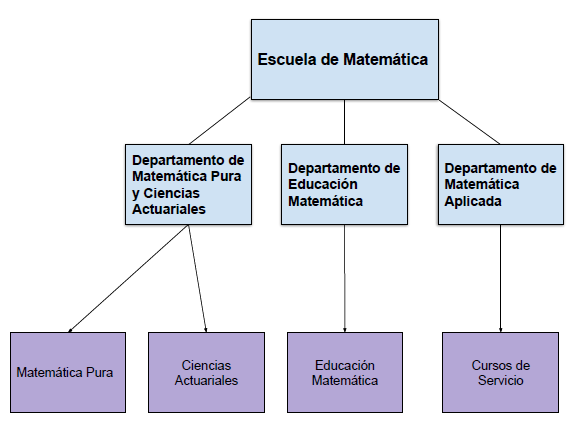
\includegraphics[width=0.5\linewidth]{dptos.png}
    \caption{División por departamentos vigente en la Escuela de Matemática}
    \label{fig:dpto}
\end{figure}

\subsection{Cuerpo docente}
En la Tabla \ref{tab:docentes} se presenta el personal docente activo que ha impartido cursos en la carrera de Matemática desde el año 2010. Se clasifican por áreas de especialización, que corresponde a la especialización que tiene más cercanía a las áreas curriculares que se definieron con anterioridad. En la última columna de la tabla se especifica si el nombramiento de cada docente es en propiedad (P), becario (B), exbecario (E), o interinazgo (I).

% Please add the following required packages to your document preamble:
% \usepackage{longtable}
% Note: It may be necessary to compile the document several times to get a multi-page table to line up properly
\begin{longtable}[c]{|l|l|c|}
\caption{Lista de docentes en condición activa que han impartido cursos desde el 2010.}
\label{tab:docentes}\\
\hline
\rowcolor[HTML]{00C0F3}
Docente & Especialidad & Nombramiento \\ \hline
%
\endhead
%
Jennifer Acuña Larios & Análisis & P \\ \hline
Luis Acuña Valverde &  & P \\ \hline
Josué Ávila Artavia &  & E \\ \hline
Luis Barboza Chinchilla &  & P \\ \hline
Adrián Barquero Sánchez &  & P \\ \hline
Raúl Bolaños Guerrero &  & P \\ \hline
Ronald Bustamante Medina &  & P \\ \hline
Juan Gabriel Calvo Alpízar &  & P \\ \hline
Santiago Cambronero Villalobos &  & P \\ \hline
José David Campos Fernández &  & P \\ \hline
Daniel Campos Salas &  & P \\ \hline
Santiago Chaves Aguilar &  & E \\ \hline
Pedro Díaz Navarro &  & I \\ \hline
Christian Fonseca Mora &  & P \\ \hline
Álvaro Guevara Villalobos &  & P \\ \hline
Jorge Guier Acosta &  & P \\ \hline
Jonathan Gutiérrez Pavón &  & P \\ \hline
Alberto Hernández Alvarado &  & P \\ \hline
David Jiménez López &  & P \\ \hline
David Krumm Cabezas &  & I \\ \hline
Allan Lacy Mora &  & P \\ \hline
Jennifer Loría Sorio &  & E \\ \hline
Darío Mena Arias &  & P \\ \hline
Pedro Méndez Hernández &  & P \\ \hline
Carlos Montalto Cruz &  & P \\ \hline
Samaria Montenegro Guzmán &  & P \\ \hline
German Mora Sáenz &  & B \\ \hline
Adrián Naranjo Alvarado &  & B \\ \hline
Hugo Peña Gómez &  & I \\ \hline
Alexander Ramírez González &  & P \\ \hline
Oldemar Rodríguez Rojas &  & P \\ \hline
José Rosales Ortega &  & P \\ \hline
Adriana Sánchez Chavarría &  & P \\ \hline
Jesús Sánchez Guevara &  & P \\ \hline
Fabio Sánchez Peña &  & P \\ \hline
Esteban Segura Ugalde &  & P \\ \hline
Filánder Sequeira Chavarría &  & I \\ \hline
Maikol Solís Chacón &  & P \\ \hline
Javier Trejos Zelaya &  & P \\ \hline
William Ugalde Gómez &  & P \\ \hline
Roberto Ulloa Esquivel &  & E \\ \hline
Mario Villalobos Arias &  & P \\ \hline
Mark Villarino Bertran &  & P \\ \hline
Rafael Zamora Calero &  & P \\ \hline
Óscar Zamora Luna &  & E \\ \hline
Ronald Zúñiga Rojas &  & P \\ \hline
\end{longtable}


Con base en la información anterior, se detalla la cantidad de profesores disponibles (no exclusivos) por cada uno de los cursos que componen la malla curricular propuesta en la Tabla \ref{tab:cursos}. Es importante agregar que muchos docentes están simultáneamente disponibles en más de un curso, por lo que esta tabla representa un escenario optimista de la cantidad de recursos disponibles en la Escuela de Matemática para hacerle frente a la oferta académica. Cada curso se espera que sea impartido por docentes con doctorado. En el caso de tener maestría, se permitirá si el  curso es relacionado con el área de trabajo. %Por otro lado, la columna que indica el grado académico mínimo es definido con respecto a la complejidad de los contenidos y a la ubicación del curso en la malla curricular.


\begin{longtable}[c]{|l|p{7cm}|p{3.4cm}|p{2cm}|}
\caption{Número de personal docente por curso del nuevo plan de estudios, según especialidad}
\label{tab:cursos}\\
\hline
\rowcolor[HTML]{00C0F3}
Sigla & Curso & Área de especialidad & Número de docentes \\ \hline
%
\endhead
%
\MA{0151} & \gls{MA0151} & General &  \\ \hline
\MA{0152} & \gls{MA0152} & General &  \\ \hline
\MA{0251} & \gls{MA0251} & General &  \\ \hline
\MA{0252} & \gls{MA0252} & General &  \\ \hline
\MA{0261} & \gls{MA0261} & Álgebra &  \\ \hline
\MA{0341} & \gls{MA0341} & Numérico &  \\ \hline
\MA{0351} & \gls{MA0351} & Análisis &  \\ \hline
\MA{0361} & \gls{MA0361} & Álgebra &  \\ \hline
\MA{0451} & \gls{MA0451} & Análisis &  \\ \hline
\MA{0461} & \gls{MA0461} & Teoría de números &  \\ \hline
\MA{0471} & \gls{MA0471} & Análisis &  \\ \hline
\MA{0472} & \gls{MA0472} & Geometría &  \\ \hline
\MA{0515} & \gls{MA0515} & Análisis &  \\ \hline
\MA{0520} & \gls{MA0520} & Análisis/Estadística &  \\ \hline
\MA{0535} & \gls{MA0535} & Álgebra &  \\ \hline
\MA{0541} & \gls{MA0541} & Numérico &  \\ \hline
\MA{0615} & \gls{MA0615} & Análisis &  \\ \hline
\MA{0625} & \gls{MA0625} & Análisis &  \\ \hline
\MA{0635} & \gls{MA0635} & Álgebra &  \\ \hline
\MA{063X} & \gls{MA063X} & Topología &  \\ \hline
\MA{0702} & \gls{MA0702} & Análisis &  \\ \hline
\MA{0725} & \gls{MA0725} & Análisis &  \\ \hline
\MA{07xx} & \gls{MA07xx} & Geometría &  \\ \hline
\MA{-OPT} & \gls{OPT-Algebra} & Álgebra &  \\ \hline
\MA{-OPT} & \gls{OPT-Analisis} & Análisis &  \\ \hline
\MA{-OPT} & \gls{OPT-Aplicada} & Aplicada &  \\ \hline
\MA{-OPT} & \gls{OPT-Computacion cientifica} & Numérico &  \\ \hline
\MA{-OPT} & \gls{OPT-Discreta} & Discreta &  \\ \hline
\MA{-OPT} & \gls{OPT-Estadistica, Ciencia datos} & Estadística&  \\ \hline
\MA{-OPT} & \gls{OPT-Geometria} & Geometría &  \\ \hline
\MA{-OPT} & \gls{OPT-Logica} & Lógica &  \\ \hline
\MA{-OPT} & \gls{OPT-Topologia} & Topología &  \\ \hline
%\end{tabular}
\end{longtable}


\subsection{Plan de Transición}
Para estudiantes activos que ingresaron en el año 2025 o anteriores, se propone un plan de transición con base en el cohorte que corresponda, bajo el supuesto de que cada estudiante tiene el año correspondiente al cohorte completo al finalizar el año 2025. 

\subsubsection{Cohorte C5}
Se estima que este grupo tendrá 50 estudiantes, quienes aprobaron MA0150 y MA0250, además de los cursos de generales de primer año. A este grupo se le debe convalidar MA0251, MA0252 y permitir que MA0261 sea correquisito con los cursos del I26, como excepción por el plan de transición.
\begin{table}[h!]
\centering
\begin{tabular}{|c|l|}
\hline
\rowcolor[HTML]{00C0F3}
Cohorte C5 & Primer año completo del plan anterior \\ \hline
I26 & \begin{tabular}[c]{@{}l@{}}MA0261 \gls{MA0261} (3)\\ MA0341 \gls{MA0341} (4)\\ MA0351 \gls{MA0351} (4)\\ Artística (2)\end{tabular} \\ \hline
II26 & \begin{tabular}[c]{@{}l@{}}MA0361 \gls{MA0361} (4)\\ MA0451 \gls{MA0451} (4)\\ MA0461 \gls{MA0461} (4)\\ MA0471 \gls{MA0471} (4)\\ Seminario de Realidad Nacional I (2)\end{tabular} \\ \hline
I27 & Igual que Ciclo V - Plan 26 \\ \hline
II 27 & Igual que Ciclo VI - Plan 26 \\ \hline
I 28 & Igual que Ciclo VII - Plan 26 \\ \hline
II 28 & Igual que Ciclo VIII - Plan 26 \\ \hline
\end{tabular}
\end{table}

\subsubsection{Cohorte C4}
Se estima que este grupo tendrá 35 estudiantes, quienes aprobaron MA0150, MA0250, MA0350, MA0360, MA0370, MA0450 y MA0460. A este grupo se le debe convalidar MA0252, MA0351, MA0341, y permitir que MA0461 y MA0535 sean correquisitos, como excepción por el plan de transición.

\begin{table}[h!]
\centering
\begin{tabular}{|l|l|}
\hline
\rowcolor[HTML]{00C0F3}
Cohorte C4 & Segundo año completo del plan anterior) \\ \hline
I26 & \begin{tabular}[c]{@{}l@{}}MA0461 \gls{MA0461} (4)\\ MA0520 \gls{MA0520} (4)\\ MA0535 \gls{MA0535} (4)\\ MA0541 \gls{MA0541} (4)\\ Seminario de Realidad Nacional II (2)\end{tabular} \\ \hline
II26 & Igual que Ciclo VI - Plan 26 \\ \hline
I27 & Igual que Ciclo VII - Plan 26 \\ \hline
II 27 & Igual que Ciclo VIII - Plan 26 \\ \hline
\end{tabular}
\end{table}

\subsubsection{Cohorte C3}
Quienes tengan tres años completos del plan anterior, deben finalizar dicho plan, para lo cual deben cursar MA0702, MA0704, MA0870 y tres optativas de Matemática.

\subsubsection{Excepciones}
Cada estudiante que no haya cumplido sus ciclos de estudio de acuerdo con el plan de estudios anterior, no contemplados en los incisos anteriores, o aquellos de planes previos, deberá de utilizar la tabla de convalidaciones para trasladarse hacia la malla del nuevo plan de estudios, y deberá cursar los cursos no convalidables hasta cumplir con todos los requisitos del plan 2026. 

\subsubsection{Convalidaciones}

Se plantea considerar las siguientes convalidaciones, para casos particulares que no cumplen con un cohorte específico; ver Tabla \ref{tab:conv}. De esta forma, se deberán trasladar al plan 2026, realizando las convalidaciones que correspondan, y deberán cursar aquellos cursos no convalidables hasta cumplir con todos los requisitos del plan 2026.

\begin{table}[h!]
\centering
\caption{Convalidaciones para transicione de plan de estudios}
\label{tab:conv}
\begin{tabular}{|p{6cm}|p{8.5cm}|}
\rowcolor[HTML]{00C0F3}
\hline
Sigla y curso aprobado & Sigla y curso por convalidar \\ \hline
MA0150 Principios de Matematica & \begin{tabular}[c]{@{}l@{}}MA0152 \gls{MA0152}\\ MA0252 \gls{MA0252}\end{tabular} \\ \hline
\begin{tabular}[c]{@{}l@{}}MA0250 Cálculo en una variable I\\ MA0350 Cálculo en una variable II\end{tabular} & \begin{tabular}[c]{@{}l@{}}MA0251 \gls{MA0251}\\ MA0451 \gls{MA0451}\end{tabular} \\ \hline
MA0450 Cálculo en varias variables & \begin{tabular}[c]{@{}l@{}}MA0351 \gls{MA0351}\\ MA0515 \gls{MA0515}\end{tabular} \\ \hline
MA0360 Álgebra lineal I & MA0261 \gls{MA0261} \\ \hline
MA0455 Ec. dif. ordinarias & MA0615 \gls{MA0615} \\ \hline
MA0460 Álgebra lineal II & MA0361 \gls{MA0361} \\ \hline
MA0501 Análisis numérico I & MA0541 \gls{MA0541} \\ \hline
MA0505 Análisis I & MA0625 \gls{MA0625} \\ \hline
MA0561 Grupos y anillos & MA0535 \gls{MA0535} \\ \hline
MA0605 Análisis II & MA0725 \gls{MA0725} \\ \hline
MA0660 Teoría de Galois & MA0635 \gls{MA0635} \\ \hline
MA0704 Topología General I & MA063X \gls{MA063X} \\ \hline
\end{tabular}
\end{table}

\subsection{Proyección de carga académica para el plan de transición}

Según el plan descrito en la sección anterior, se presenta la proyección de carga académica necesaria para suplir la demanda de los años de transición (2026, 2027, 2028). Esto bajo el supuesto de recibir el máximo de 26 estudiantes por año más doce estudiantes por traslado, ofertando dos grupos por curso en primer año.

\begin{longtable}[c]{|l|l|l|l|l|l|}
\caption{Proyección de carga académica para el plan de transición, año 2026}
\label{tab:carga2026}\\
\hline
\rowcolor[HTML]{00C0F3}
Ciclo & Cohorte & Curso & Créditos & Grupos & Jornada \\ \hline
\endhead
%
I & C3 & MA0702 & 5 & 1 & 0.375 \\ \hline
I & C3 & MA0704 & 5 & 1 & 0.375 \\ \hline
I & C3 & MA OPT & 5 & 1 & 0.375 \\ \hline
I & C4 & MA0461 & 4 & 1 & 0.375 \\ \hline
I & C4 & MA0520 & 4 & 1 & 0.375 \\ \hline
I & C4 & MA0535 & 4 & 1 & 0.375 \\ \hline
I & C4 & MA0541 & 4 & 1 & 0.375 \\ \hline
I & C5 & MA0261 & 3 & 1 & 0.375 \\ \hline
I & C5 & MA0341 & 4 & 1 & 0.375 \\ \hline
I & C5 & MA0351 & 4 & 1 & 0.375 \\ \hline
I & C6 & MA0151 & 3 & 2 & 0.375 \\ \hline
I & C6 & MA0152 & 3 & 2 & 0.375 \\ \hline
I & C6 & Inglés I & 3 & 2 & 0.250 \\ \hline
 &  & 14 3/8 & 2 2/8 & Total & 5.750 \\ \hline
II & C3 & MA0870 & 5 & 1 & 0.375 \\ \hline
II & C3 & MA OPT & 5 & 1 & 0.375 \\ \hline
II & C3 & MA OPT & 5 & 1 & 0.375 \\ \hline
II & C4 & MA063X & 4 & 1 & 0.375 \\ \hline
II & C4 & MA0615 & 4 & 1 & 0.375 \\ \hline
II & C4 & MA0625 & 4 & 1 & 0.375 \\ \hline
II & C4 & MA0635 & 4 & 1 & 0.375 \\ \hline
II & C4 & Módulo 1 & 2 & 1 & 0.250 \\ \hline
II & C5 & MA0361 & 4 & 1 & 0.375 \\ \hline
II & C5 & MA0451 & 4 & 1 & 0.375 \\ \hline
II & C5 & MA0461 & 4 & 1 & 0.375 \\ \hline
II & C5 & MA0471 & 4 & 1 & 0.375 \\ \hline
II & C6 & MA0251 & 3 & 2 & 0.375 \\ \hline
II & C6 & MA0252 & 3 & 2 & 0.375 \\ \hline
II & C6 & MA0261 & 3 & 2 & 0.375 \\ \hline
II & C6 & Inglés II & 3 & 2 & 0.250 \\ \hline
 &  & 17 3/8 & 3 2/8 & Total & 7.125 \\ \hline
\end{longtable}

% Please add the following required packages to your document preamble:
% \usepackage{longtable}
% Note: It may be necessary to compile the document several times to get a multi-page table to line up properly
\begin{longtable}[c]{|l|l|l|l|l|l|}
\caption{Proyección de carga académica para el plan de transición, año 2027}
\label{tab:carga2027}\\
\hline
\rowcolor[HTML]{00C0F3}
Ciclo & Cohorte & Curso & Créditos & Grupos & Jornada \\ \hline
\endhead
%
I & C4 & Módulo 2 & 2 & 1 & 0.250 \\ \hline
I & C4 & MA07XX & 4 & 1 & 0.375 \\ \hline
I & C4 & MA0702 & 4 & 1 & 0.375 \\ \hline
I & C4 & MA0725 & 4 & 1 & 0.375 \\ \hline
I & C4 & MA OPT & 4 & 1 & 0.375 \\ \hline
I & C5 & MA0515 & 4 & 1 & 0.375 \\ \hline
I & C5 & MA0520 & 4 & 1 & 0.375 \\ \hline
I & C5 & MA0535 & 4 & 1 & 0.375 \\ \hline
I & C5 & MA0541 & 4 & 1 & 0.375 \\ \hline
I & C6 & MA0341 & 4 & 1 & 0.375 \\ \hline
I & C6 & MA0351 & 4 & 1 & 0.375 \\ \hline
I & C6 & MA0361 & 4 & 1 & 0.375 \\ \hline
I & C6 & Inglés III & 3 & 2 & 0.250 \\ \hline
I & C7 & MA0151 & 3 & 2 & 0.375 \\ \hline
I & C7 & M10152 & 3 & 2 & 0.375 \\ \hline
I & C7 & Inglés I & 3 & 1 & 0.250 \\ \hline
 &  & 15 3/8 & 4 2/8 & Total & 6.625 \\ \hline
II & C4 & MA OPT & 4 & 4 & 0.375 \\ \hline
II & C4 & Módulo 3 & 2 & 1 & 0.250 \\ \hline
II & C5 & Módulo 1 & 2 & 1 & 0.250 \\ \hline
II & C5 & MA063X & 4 & 1 & 0.375 \\ \hline
II & C5 & MA0615 & 4 & 1 & 0.375 \\ \hline
II & C5 & MA0625 & 4 & 1 & 0.375 \\ \hline
II & C5 & MA0635 & 4 & 1 & 0.375 \\ \hline
II & C6 & MA0451 & 4 & 1 & 0.375 \\ \hline
II & C6 & MA0461 & 4 & 1 & 0.375 \\ \hline
II & C6 & MA0471 & 4 & 1 & 0.375 \\ \hline
II & C6 & MA0472 & 4 & 1 & 0.375 \\ \hline
II & C7 & MA0251 & 3 & 2 & 0.375 \\ \hline
II & C7 & MA0252 & 3 & 2 & 0.375 \\ \hline
II & C7 & MA0261 & 3 & 2 & 0.375 \\ \hline
II & C7 & Inglés 2 & 3 & 1 & 0.250 \\ \hline
 &  & 18 3/8 & 3 2/8 & Total & 7.500 \\ \hline
\end{longtable}

A las cargas anteriores, debe de sumarse la carga por rezago en cursos. Históricamente, se han abierto los cursos de matemática de los dos primeros años de forma permanente, por lo que en la Tabla \ref{tab:resumenCarga} se contabiliza dicha carga.
%En II25 se debe sumar carga por cursos de primer y segundo año repitentes
\begin{longtable}[c]{|c|c|c|c|}
\caption{Carga proyectada total del plan de transición}
\label{tab:resumenCarga}\\
\hline
\rowcolor[HTML]{00C0F3}
Ciclo & Carga plan de transición & Carga adicional por rezago & Carga total proyectada \\ \hline
\endhead
%
I26 & 5.750 & 0 & 6.750 \\ \hline
II26 & 7.125 & 1.875 & 9.000 \\ \hline
I27 (y posteriores) & 6.625 & 2.625 & 9.250 \\ \hline
II27 (y posteriores) & 7.500 & 1.875 & 9.375 \\ \hline
\end{longtable}

\section{Seguimiento y Evaluación}

En esta sección se plantea la estrategia de evaluación de la carrera y el plan de desarrollo docente que la Escuela de Matemática podría implementar para capacitar al cuerpo docente ante las nuevas exigencias académicas de la malla propuesta.

\subsection{Momentos y estrategias de evaluación de la carrera}

La puesta en marcha de esta propuesta estará a cargo de la persona directora del Departamento de Matemática, en conjunto con la comisión que elaboró esta propuesta, quienes supervisarán la implementación completa del proceso de transición y la asignación y ejecución de carga presupuestaria tal y como se detalla en la Sección 5.1. Asimismo, será el Departamento de Matemática el encargado de ejecutar las estrategias de desarrollo docente que se explican en la siguiente sección, preferiblemente a través de la conformación de una comisión con ese objetivo en particular. 
Por otro lado, se recomienda que el Departamento nombre una comisión encargada de la evaluación de la malla curricular propuesta para que tenga listo un diagnóstico del perfil de salida y de la malla vigente a lo sumo cinco años después de que el plan se haya incorporado de manera completa en la población estudiantil. Se recomienda que los mismos miembros que conformaron la elaboración de este documento participen en esa comisión de evaluación.

\subsection{Desarrollo docente}

\subsection{Presupuesto}
